\chapter{Background}
\label{background}

	In computer security, intrusion detection is the fact of detecting malicious actions that attempt to compromise the confidentiality, integrity or availability of a resource. Intrusion detection can be performed manually or automatically.\ In the process of manual intrusion detection, a human examines log files to find any suspicious sign that can indicate an intrusion.\ A system that performs the automated intrusion detection is called intrusion detection system (IDS).

	In this chapter, we will take a deeper look on the Intrusion detection systems. We will explain the possible categories of those systems in the first section, present the available datasets to evaluate them in the second section and give a brief overview of the algorithms used in our project in the remaining sections.

	\section{Intrusion detection systems (IDS)}

		An intrusion detection system is a mechanism intended to analyse the security status of an information system in order to detect anomalies or suspicious activities.

		\subsection{Typical Components }

			As described in \cite{BSI}, the software components of an Intrusion Detection System can be be grouped, according to their functions, into four types:

			\begin{description}
				\item[- Sensors:] They are responsible for collecting  events from host or network-based data sources and transmitting them for further analysis and storage.

				\item [- Evaluation stations:] They analyze the events and identify the attacks. The evaluated informations will be also transmitted as events, which allows repeated analysis. 
				\item [- Management stations:] They regulate the communication between the individual components of an IDS, determine the necessary parameters, monitor the individual event streams and send warning messages.
				\item [- Database Components:] They are used to efficiently manage and store the collected data of all components.

			\end{description}

		\subsection{IDS Taxonomy}

			As presented in figure \ref{Taxonomy of intrusion detection systems}, IDS systems could be classified into four categories.

			\begin{figure}[h!]
				\centering
				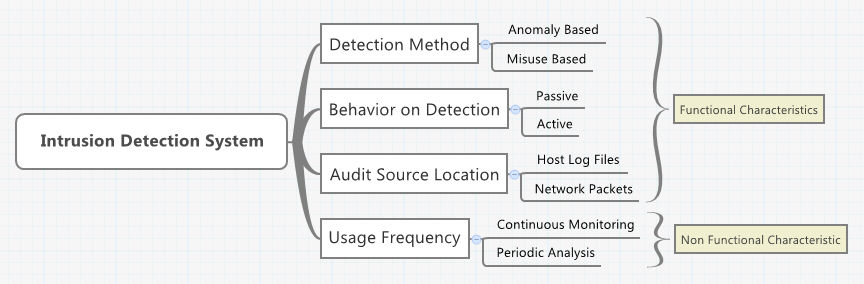
\includegraphics[scale=0.45]{figures/Taxonomy.png}
				\caption{Taxonomy of intrusion detection systems}
				\label{Taxonomy of intrusion detection systems} 	
			\end{figure}
				
			The network security tool uses either of two main approaches to detect the anomalies.\ The first one, anomaly based, explores issues in intrusion detection associated with deviations from normal behaviour of the monitored system.\ The second approach uses informations about attacks to discriminate between anomaly or attack patterns.\ After detecting an attack, an active IDS tool can automatically block suspected attacks in progress (known as an intrusion response system), whereas a passive IDS can only alert an operator to potential vulnerabilities and attacks and log network packets.

	
			Intrusion detection systems can be classified according to the source of data.\ An IDS tool can either use informations derived from a single host: host based IDS (HIDS) and or exploit informations obtained from a whole segment of a local network (network based IDS, i.e. NIDS).


			An IDS tool can be characterized by its usage frequency, we distinguish between a dynamic IDS that runs on a continuous feed of information and performs real-time analysis and a static IDS that periodically takes a snapshot of the environment and analyzes it.


		\subsection{Detection Methodologies}

			In this section we discuss the primary classes of detection methodologies: Misuse-based based and Anomaly based.

			\subsubsection{Misuse-based intrusion detection}

				The Misuse-based intrusion detection system possesses patterns describing known attacks called signatures.\ It is the simplest detection method as it identifies possible attacks by just comparing those signatures against observed events. 


				While these systems are very effective at uncovering known attacks with a few number of false alarms, they are not able to detect novel attacks for which the signatures are not yet available, therefore the signatures must be constantly updated.\ Two approaches are commonly used to implement this technique: 

				\begin{description}

					\item[\textbf{- Pattern matching approach:}] In this approach attack patterns are modelled, matched and identified based on the packet header and/or packet content.
					\item[\textbf{- Rule-based approach:}] This approach makes use of expert systems that contain a set of rules describing the attacks, which are matched against audit or network traffic data.\ Any deviation in the rule matching process is reported as an intrusion.

				\end{description}
	
			\subsubsection{Anomaly detection} 

				Anomaly detection constructs normal activity profiles for the system during a training phase and then considers any current behavior that does not match the stored profile as a suspicious action.\ These systems are able to detect novel attacks, but they generally have a substantial false alarm rate and the training of a very dynamic system requires a constant update of the normal behaviour profile database.\ According to \cite{AnomalyBasedNID} anomaly detection techniques can be grouped into three main approaches:

				\begin{description}
					\item[\textbf{- Statistical-based techniques:}] A user or a system profile reflecting its behavior is constructed by measuring a number of variables sampled over time.
					\item[\textbf{- Knowledge based techniques:}] They require the availability of prior knowledge. The expert system approach is one of the most widely used Knowledge based schemes.
					\item[\textbf{- Machine Learning techniques :}] They are widely used in the anomaly based intrusion detection since they enable to automatically construct a model that reflects the subject's normal behavior. They fall into two categories: supervised and unsupervised learning.

						\begin{itemize}
							\item { \textbf{Supervised learning:}} It proceeds in two steps, first in the training phase a classification model is learned based on datasets labeled with predefined classes . Then, in the testing phase, ths classification model is used to predict the classes of new instances. SVM, neural networks, Bayesian network are some of the widely used supervised learning techniques. Section \ref{svmSection} will be dedicated to better explain the support vector machines.
							\item { \textbf{Unsupervised learning:}} They try to detect intrusions without using any prior knowledge of attacks or normal instances.\ Clustering and outlier detection based techniques are among the most popular approaches suggested.\ Among the clustering strategies we find the K-means approach which will be further discussed in section \ref{kmeans}.

						\end{itemize}
				\end{description}

			\subsection{Data source locations} 
				
				Intrusion detection systems can be categorised into two groups based on the location of the data source: network-based IDS or host-based IDS.

				\subsubsection*{Host based IDS}

					In this case, informations on the activities of the users of a given machine are gathered based only on the Host audit sources, for example: system commands like: \textit{vmstat}, \textit{pstat}; Syslog audit service.
				 
				\subsubsection*{Network based IDS}

					A network-based IDS collects informations from the network traffic streams  as data is transmitted between particular network segments, suspicious activities are identified inspecting the contents and header informations of all the packets transferred across those segments.\ In the following we'll give a brief overview of the TCP/IP protocol suite and then we will cover the major components of network-based IDSs.

					\begin{enumerate}
						\item{\textbf{Transmission Control Protocol}}
						
							To provide network communication the internet protocol stack is composed of 4 layers: the data link, network, transport, and application layers.\ When a user wants to transfer data across networks, the data is passed through all the layers starting from the application layer, with each layer encapsulating  more header informations.\ The data link layer sends the packet through the physical network; when received by a host the data gets decapsulated as it is passed up  through the layers.

							The TCP protocol is a connection oriented transport protocol, that is, the sender and the receiver processes must handshake with each other by exchanging control messages initialzing many state variables contained in the TCP header before establishing the connection.

							Figure \ref{tcp} depicts the TCP headers as defined in RFC 793.
								\begin{figure}[h!]
									\centering
									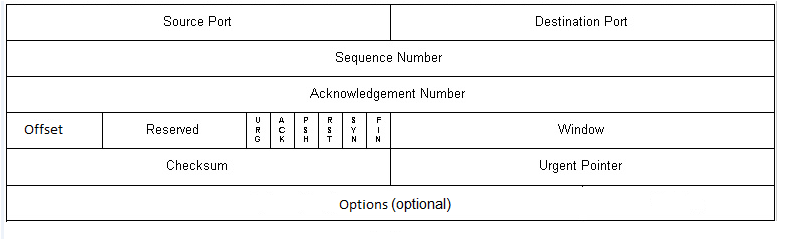
\includegraphics[scale=0.66]{figures/TCP.png} 
									\caption{TCP Header}\label{tcp} 	
								\end{figure}

							The source and destination ports contain respectively the source and the destination port number of the packet.\ For each TCP connection, numbers are negotiated between the communication partners.\ The sequence number field contains the number of first byte in segment's data.\ The acknowledgment number is the sequence number of the next byte expected from the other side, thus the sender can determine whether the data arrived at the receiver.
							
					\begin{table}[h!]
						\centering
  						\resizebox{\textwidth}{!}{ 						
							\begin{tabular}{|c|c|p{6cm}|}
								\hline 
								\textbf{Flag} & \textbf{Meaning} & \textbf{Function} \\ 
								\hline 
								$URG$ & Urgent & Set if data is urgent \\ 
								\hline 
								$ACK$ & Acknowledgment & Acknowledges the received data \\ 
								\hline 
								$PSH$ & Push & Informs the receiving host that the data should be immediately pushed up to the receiving application  \\ 
								\hline 
								$RST$ & Reset & Reset the connection in response to an invalid segment \\ 
								\hline 
								$SYN$ & Synchronise & Initiates a connection \newline
								$SYN$ = 1, $ACK$ = 0 for connection request;\newline 
								$SYN$ = 1, $ACK$ = 1 for acknowledgment of receipt\\ 
								\hline 
								$FIN$ & Finish & Closes a connection\newline
								$FIN$ = 1, ACK = 0 Disconnection request;\newline 
								$FIN$ = 1, ACK = 1 Confirmation \\ 
								\hline 
							\end{tabular} 
						}
								\caption{TCP Flags} \label{flags}
						\end{table}				

						\item {\textbf{Architecture overview:}}\\
						
							The network IDS usually has two logical components: the sensors and the management station \cite{guide}.\\
							
							\begin{description}
								\item[- The sensors:] They are on the network segments, they are dedicated to monitor them for suspicious traffic.\ Their network interface is set in the promiscuous mode, which means they receive all network traffic.\ If they detect a suspicious packet, they send it to the management station.
								\item[- The management station:] It receives alarms from the sensor(s), stores them in the Simple Network Management Protocol (SNMP) Management Information Base (MIB).\ It can perform some additional analysis and display them to the network administrator.
							\end{description}

							The placement of the sensors and the management station is shown in Figure~\ref{archi}.

							\begin{figure}[h!]
								\centering
								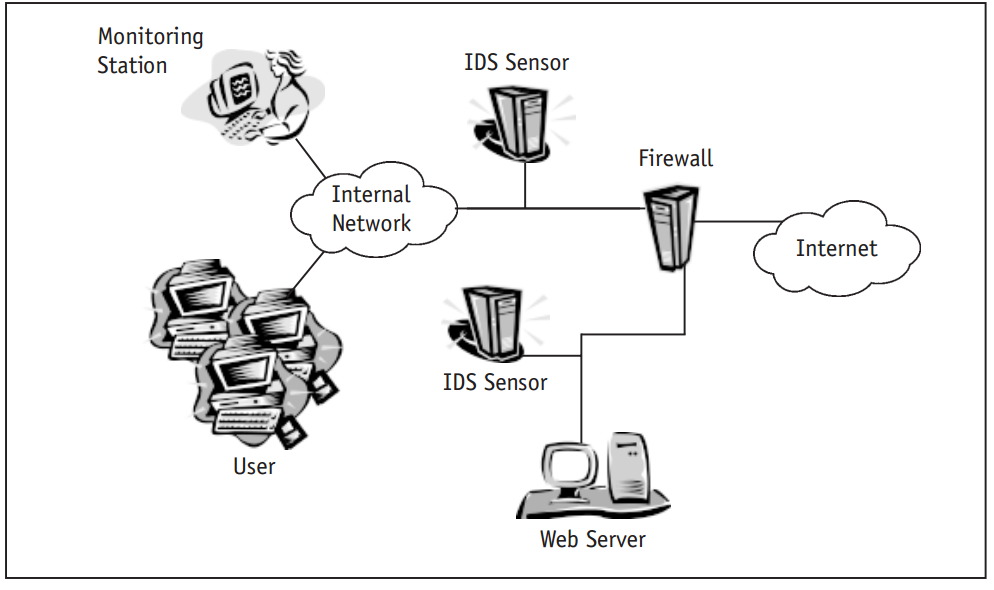
\includegraphics[scale=0.5]{figures/NIDS.PNG} 
								\caption{Network based IDS architecture \cite{guide}}
								\label{archi} 
							\end{figure}
					\end{enumerate}
		
		\section{Available Datasets} 

			Datasets are utilized to evaluate the performance of Intrusion Detection Systems.\ There are two publicly available datasets: The DARPA datasets developed by the MIT Lincoln Labs and the KDD Cup dataset derived from them, they both consist of US air force local network data with a variety of simulated attacks.

				\subsection{DARPA Datasets}
				
					The DARPA datasets were built by MIT Lincoln Laboratory in 1998 and 1999 in the context of a project supported by DARPA aiming to provide a source of data that enables to quantitatively evaluate Intrusion detection systems.\ They performed a simulation of an Air Force base connected to the Internet.

					The 1999 Off-line Simulation Network architecture is depicted in figure \ref{DARPA archi}.\ As shown in the figure, the simulation network has two segments where the left side represents the networks inside of the simulated Eyrie Air Force Base, it includes victim machines with different operating systems and a gateway to other inside workstations and the right side represents the Internet outside the base. 

					\begin{figure}[h!]
						\centering
						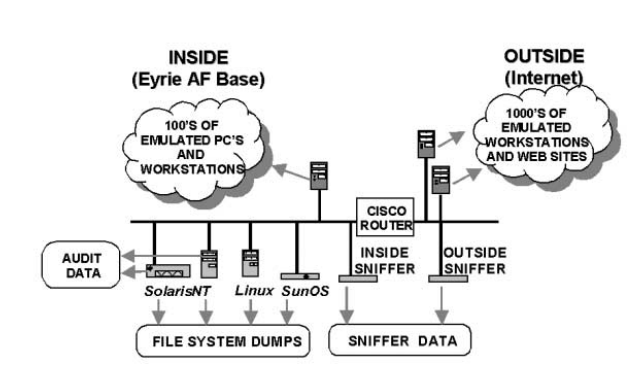
\includegraphics[scale=0.7]{figures/Network.PNG}
						\caption{DARPA'$99$ simulation network architecture}
						\cite{DARPAEvaluation}
						\label{DARPA archi}	
					\end{figure}
						
					The test bed network generated three weeks of training data with background traffic and labeled attack, the first and third weeks of the training data can be used in the training of anomaly detection systems as they do not contain any attacks, and two weeks of test data with background traffic and unlabelled attacks.\ The attacks used in the simulations can be divided into four categories \cite{ComparativeStudy}, namely:

					\begin{itemize}
						\item {Probing:} Attacks that attempts to gather information about network of computers or find known vulnerabilities.
						\item {Denial of Service (DoS):} Attacks that deny legitimate requests from legal users on the system by making full usages of computing or memory resources.
						\item {User to Root (U2R):} Attacks that exploit the vulnerability of the system to obtain root access to it from a normal user privilege.
						\item {Remote to Local (R2L):} Attacks that exploits the vulnerability of the system to gain a local user account launching remote exploits.
					\end{itemize}
					
					The procedures used in building the dataset and in performing the evaluation were criticized by MacHugh \cite{DARPACritique}.

				\subsection{KDD Dataset}

					The KDD dataset is a labeled version of 1998 MIT DARPA dataset where data packets forming a complete session were gathered in a single feature vector.\ KDD records have 41 features, defined for each connection samples which can further be classified into three groups namely: basic features, traffic features, content features \cite{Mahbod:KDD}.\ The goal of this dataset was to demonstrate the applicability of different knowledge discovery and machine learning techniques on intrusion detection systems.

		\section{Principal Component Analysis}

			Principal Components Analysis is a technique introduced by Pearson and Hotelling that aims to reduce the dimensionality of multivariate data while preserving as much as possible of the present variation.

			It is an unsupervised learning approach that only relies on the input data.\ PCA transforms a large number of variables to a new reduced set of variables, the principal components, that are uncorrelated and linear functions of the original variables, such that, the greatest variance by any projection of the data comes to lie on the first coordinate, the second greatest variance on the second coordinate, and so on.
			
			In practice, this is achieved by computing the covariance matrix for the full data set.\ Next, the eigenvectors and eigenvalues of the covariance matrix are computed, and sorted according to decreasing eigenvalue.\ This approach can be inappropriate for some applications as features with low variance might actually have high predictive relevance \cite{pca}.

		\section{Support Vector Machines}
		\label{svmSection}

			SVMs have been introduced in 1992 at the COLT conference by Boser, Guyon, Vapnik as a supervised learning approach used to solve classification and regression problems.

			The simplest kind of support vector machines called Linear SVM aims to find a hyperplane that optimally separates the training vectors into two classes by achieving the maximum separation, such that it will be equidistant to both datasets.\ Support vectors are defined to be a subset of the training data having the minimum distance to the hyperplane.\ An example of a simple linear SVM is illustrated in Figure~\ref{svm}.
				
				\begin{figure}[h!]
					\centering
					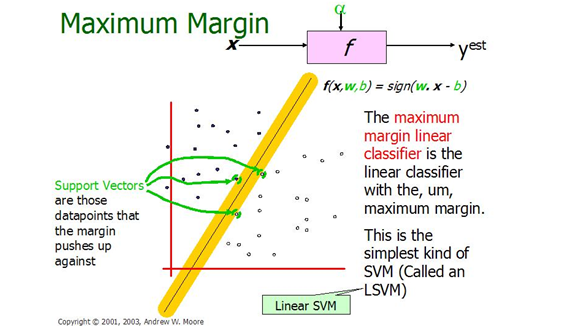
\includegraphics[scale=0.7]{figures/LSVM.PNG} 
					\caption{Linear Support Vector Machines \cite{SvmSlides}} \label{svm} 
				\end{figure}

			The goals of SVM are separating the data with a hyper plane and extend this to non-linear boundaries when the data is far from linear and the datasets are inseparable by using the kernel methods that allow SVMs to form nonlinear boundaries, by non-linearly mapping the input data to a high-dimensional space.\ The new mapping is then linearly separable \cite{Nello:Svm} \cite{Tom:MachineLearning}.

			The kernel functions enable operations to be performed in the input space rather than the potentially high dimensional feature space.\ Various kernel functions can be used \cite{Nello:Svm}, such as: \textit{Polynomial}, \textit{Gaussian Radial Basis Function}, as well as \textit{Exponential Radial Basis Function}.

			\subsection{One Class SVM}
		
			One Class SVM is an extension of the SVM methodology that handles training using only positive information, it identifies "outliers" amongst the positive examples and use them as negative examples \cite{Larry:OCSVM}. The OC-SVM algorithm maps input data into a high dimensional feature space using a kernel function and iteratively finds the maximal margin hyperplane which best separates the training data from the origin. It may be viewed as a regular two-class SVM where all the training data lies in the first class, and the origin is taken as the only member of the second class. Thus, the hyperplane (or linear decision boundary) corresponds to the classification rule. The decision function is given by:  \cite{Katherine:OCSVM}:

			\begin{equation}
				f(x) = <w,x> +b
			\end{equation}
			
			where \textit{w} is a vector perpendicular to the hyperplane and \textit{b} is a bias term. The OC-SVM solves an optimisation problem to find the decision function $f$ with maximal geometric margin.\ This function can be used to label a test example x as an anomaly if $[f(x)<0]$ and as normal otherwise. Solving the OC-SVM optimisation problem is equivalent to solving the dual quadratic programming problem:

			\begin{equation}
				\min_{\alpha} \frac{1}{2}\sum_{i,j}\alpha_{i}\alpha_{j}K(x_{i},x_{j})
			\end{equation}

			subject to the constraints

			\begin{equation}
				0 \leq \alpha_{i} \leq \frac{1}{v_{l}}
			\end{equation}
			
			and 
		
			\begin{equation}
				\sum_{i}\alpha_{i}=1
			\end{equation}

			where $\alpha_{i}$ is a Lagrange multiplier (or "weight" on example \textit{i} such that vectors associated with non-zero weights are called "support vectors" and solely determine the optimal hyperplane), \textit{v} is a parameter that controls the trade-off between maximising the distance of the hyperplane from the origin and the number of data points contained by the hyperplane, \textit{l} is the number of points in the training dataset, and $K(x_{i},x_{j})$ is the kernel function.\ Given a feature map:

			\begin{equation}
				\phi: X \longrightarrow \Re^{N}
			\end{equation}

			where $\phi$ maps training vectors from input space \textit{X} to a high dimensional feature space, the kernel function can be defined as:

			\begin{equation}
				K(x,y) = <\phi(x),\phi(y)>
			\end{equation}

			After solving for the dual problem, a set of model weights $\alpha_{i}$ can be obtained and the decision function for any test vector x can be given by :

			\begin{equation}
				f(x) = sgn (\sum_{i}\alpha_{j}K(x_{i},x_{j}) - \rho)
			\end{equation}
			
			where $\rho$ is the distance to the origin.

		\section{KMeans} \label{kmeans}

			Kmeans is an unsupervised learning algorithm that aims to organise data from a given training set into few clusters.\ The Kmeans algorithm proceeds in two steps: First $K$ data items from the set of data points are randomly chosen as initial centroids, then, in the second step, each data point is assigned to the cluster which has the closest centroid and each cluster centroid is moved to the mean of the points assigned to it.\ This second step is repeated until all data points are assigned to one of the $K$ clusters.

			The Kmeans algorithm proceeds in two steps: First K data items from the set of data points are randomly chosen as initial centroids, then, in the second step, each data point is assigned to the cluster which has the closest centroid and each cluster centroid is moved to the mean of the points assigned to it. This second step is repeated until all data points are assigned to one of the K clusters. \\

			\textbf{- Silhouette Value:}
			
				A silhouette is a graphical display for partition techniques which shows  which objects lie  well within their cluster, and which not. The average silhouette width provides an evaluation  of clustering validity and might be used to select an 'appropriate' number of clusters \cite{silhouette}.\\
			 For each data point $i$, the silhouette $s(i)$ is given by the equation \ref{SilEq}:
				
				\begin{equation} 
					s(i)=\frac{b(i)-a(i)}{\max(a(i),b(i))} 
					\label{SilEq}
				\end{equation}
						
				where $a(i)$ is the average dissimilarity of $i$ with all other data within the same cluster and $b(i)$ is the lowest average dissimilarity of $i$ to any other cluster, of which $i$ is not a member.